% $Id$

\chapter{CUTS Logging Facilities}
\label{chap:logging}

This chapter discusses the CUTS logging facilities. These facilities
are designed to simplify collection of system execution traces in 
a distributed environment. Moreover, the facilities simplify partitioning
system execution traces with different tests. This therefore makes it
possible to execute multiple tests in the same environment while 
preserving data integrity. Finally, the logging facilities discussed in
this chatper are extensible via intercepters, and are highly configurable 
so they adapt to different application domains.

\section{Overview}
\label{sec:logging-overview}

Distributed systems consist of many software components executing on
many hosts that are connected via a network. When validating distributed
system function and quality-of-service (QoS) properties, \textit{e.g.},
end-to-end response time, scalability, and throughput, it is necessary
to collect data about the systems behavior in the target environment.
Such behaviors could be the events executed of the execution lifetime of
the system, the state of the system at different points in time, or data 
points needed to calculate the end-to-end response of an event.

When dealing with data collection in a distributed environment, such 
as those that host distributed systems, data is collected and analyzed
either \textit{offline} or \textit{online}. In offline collection and 
analysis, data from each host is written to local persistent storage, 
such as a file, while the system is executing in its target environment. 
After the system is shutdown, the collected data in local storage on each 
host is combined and analyzed. The advantage of this approach is network 
traffic is kept to a minimum since collected data is not transmitted over
the network until after the system is shutdown. The disadvantage of this 
approach is collected data is not processed until the system is shutdown.
This can pose a problem for systems with a long execution lifetime, 
\textit{e.g.}, ultra-large-scale systems that must run 24x7, or when 
trying to monitor/analyze a system in real-time using collected data.

In online collection and analysis, data is collected and transmitted 
via network to a host outside the execution environment. The advantage 
of this approach is that it allows analysis of metrics data an environment 
that does not use the systems resources. This also helps not to skew the 
results while the system is running. The disadvantage of online collection
and analysis is the difficulty of devising a strategy for efficiently collecting 
data in a distributed environment and submitting it to a central location 
without negatively impacting the excuting systems QoS---especially if the
system generates heavy network traffic.
\begin{figure}[htbp]
  \centering
  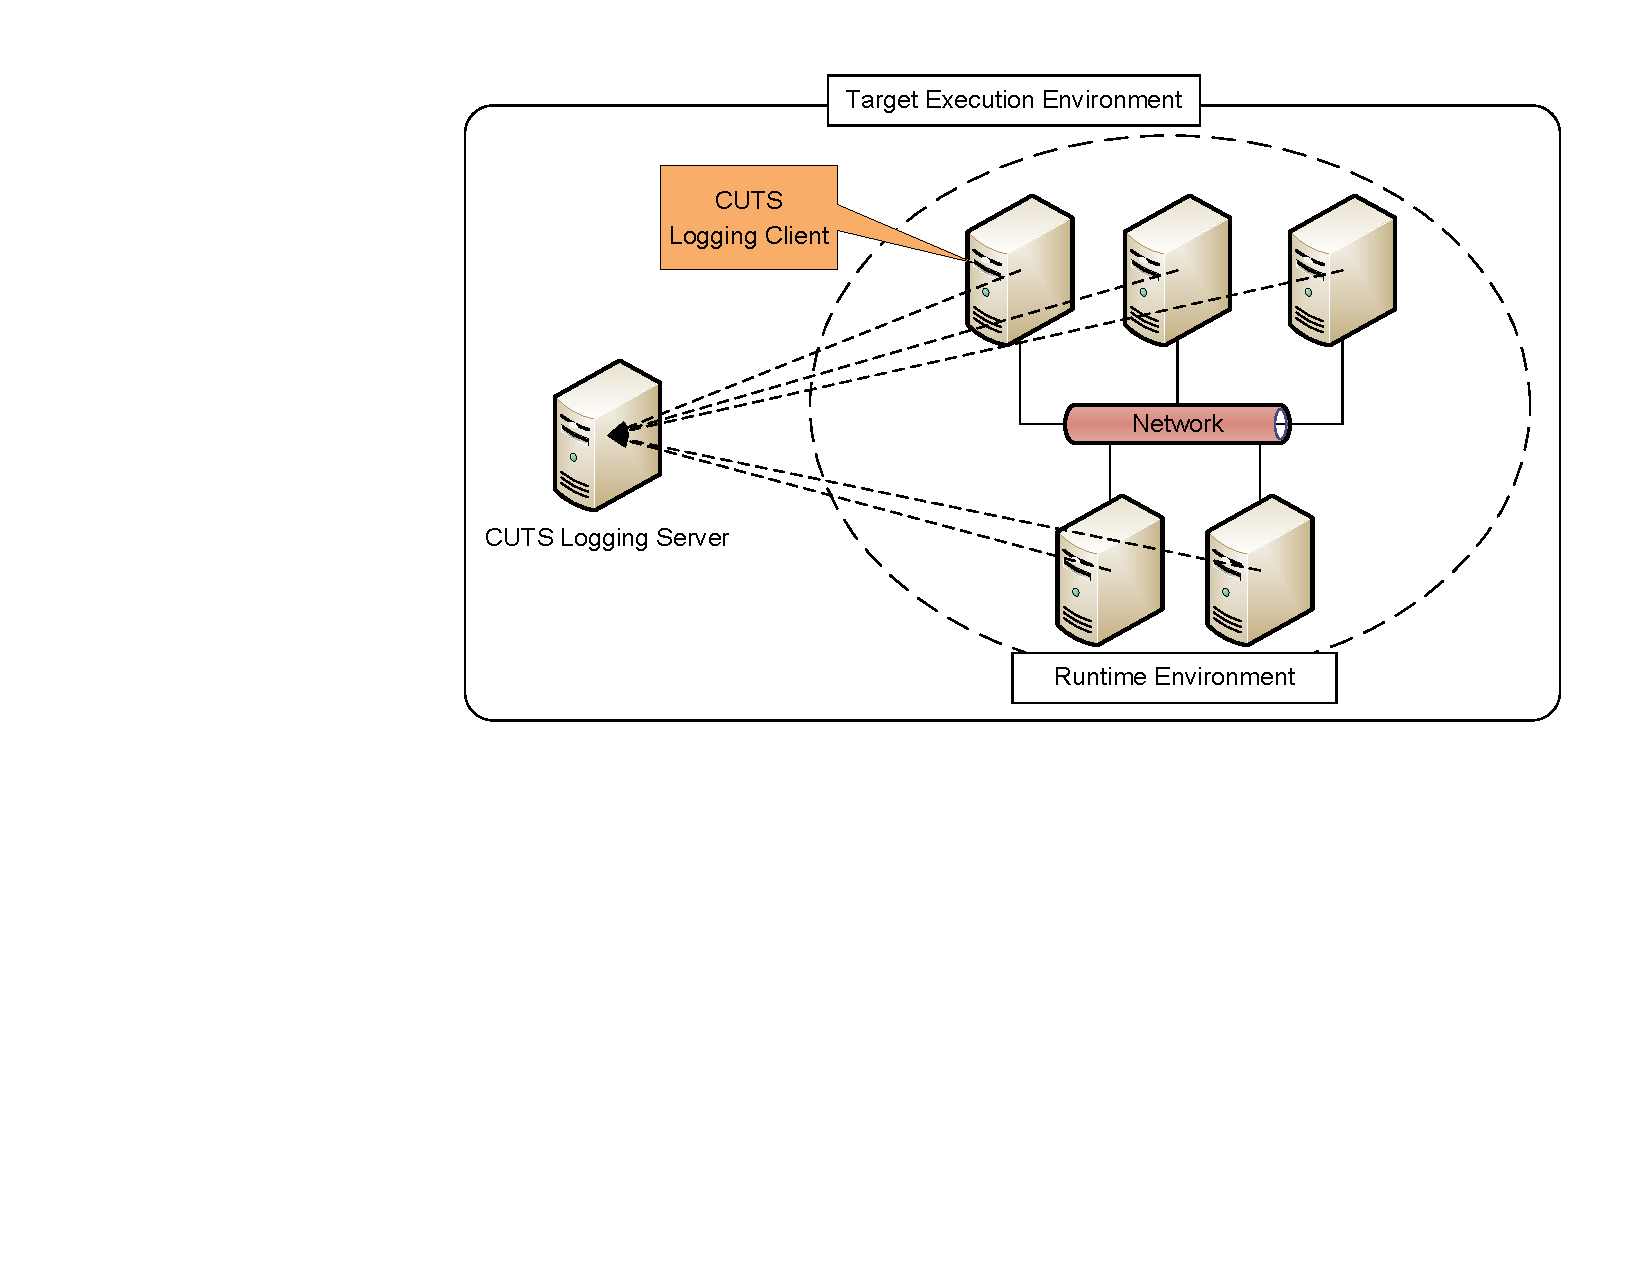
\includegraphics[scale=0.6]{logging-overview.pdf}
  \caption{Overview of the CUTS logging facilities.}
  \label{fig:logging-overview}
\end{figure}

Because online collection and analysis is a more promising approach to 
data collection and analysis, CUTS logging facilities implement online
data collection. As illustrated in Figure~\ref{fig:logging-overview},
there is a target execution environment and a runtime environment. The
runtime environment is where the system is executing and generating
data for collection. Each host in the runtime environment has a logging
client (see Section~\ref{sec:logging-client}). The logging client is 
responsible for collecting data from individual software/hardware components 
on its host. After collecting data on the host, the logging client 
periodically submits collected data to a logging server (see 
Section~\ref{sec:logging-server}), which is executing outside of 
the runtime environment.

The remainder of the chapter therefore presents the basics for
using the CUTS logging facilities in a production-like environment.
In particular, the following information is covered in this 
chapter:
\begin{itemize}
  \item \textbf{CUTS Logging Server} - The CUTS Logging Server is
  responsible for collecting data from individual CUTS Logging 
  Clients executing in the runtime environment. Details of the
  CUTS Logging Server are presented in Section~\ref{sec:logging-server}.

  \item \textbf{CUTS Logging Client} - The CUTS Logging Client is
  responsible for collecting data from individual client loggers and
  submitting it to the CUTS Logging Server. Details of the
  CUTS Logging Client are provided in Section~\ref{sec:logging-client}.

  \item \textbf{Client Logger} - The client logger is responsible for 
  collecting actual data from the runtime environment and submitting 
  it to the CUTS Logging Client executing on its host. Details of 
  the client logger are provided in Section~\ref{sec:client-loggers}.
\end{itemize}


\section{The Logging Server}
\label{sec:logging-server}

The logging server is responsible for collecting data from individual 
logging clients in the runtime environment (see Section~\ref{sec:logging-client}).
As shown in Figure~\ref{fig:logging-overview}, there is typically 
one instance of a logging server running in the target execution 
environment. There can also be cases when more than one instance of a 
logging server is desired, such as using multiple logging servers to 
balance the workload due to the amount of data collected by individual
logging clients in the runtime environment. This user's manual, however, 
assumes that only a single instance of a logging server is used in the 
runtime environment.

\subsection{Running the Logging Server}

Assuming the CUTS runtime architecture has been built and installed 
correctly, the CUTS Logging Server is installed at the following 
location:
\begin{lstlisting}
(*@\texttt{\%> \$CUTS\_ROOT/bin/cuts-logging-server}@*)
\end{lstlisting}
To see a complete list of command-line options, use the following 
command:
\begin{lstlisting}
(*@\texttt{\%> \$CUTS\_ROOT/bin/cuts-logging-server --help}@*)
\end{lstlisting}

\subsection{Configuring the Logging Server}

There are only a handful of command-line options for configuring the
logging server. The most important of the available command-line options,
is \texttt{--register-with-iortable=NAME}, where \texttt{NAME} 
is an user-defined name, such as \texttt{MyLoggingServer}. When this 
option is combined with the \texttt{-ORBEndpoint ENDPOINT} CORBA 
command-line option, an external reference to the logging server is 
created. This is what allows the CUTS Logging Client (see 
Section~\ref{sec:logging-client}) to connect to the logging server.

The following is an example of exposing the logging server on
port 20000 for logging clients to connect:
\begin{lstlisting}
(*@\texttt{\%> \$CUTS\_ROOT/bin/cuts-logging-server -ORBEndpoint}@*) \
   (*@\texttt{iiop://`hostname`:20000 --register-with-iortable=LoggingServer}@*)
\end{lstlisting}
As shown in the example above, the logging server is listening on 
port 20000 on its host~\footnote{`hostname` is used because it is assumed
that Unix command-line substitution is available on the host in the 
example. If such a feature is not available, it is possible to hardcode 
the hostname in place of `hostname`, \textit{e.g.}, host.foo.bar.com}, 
and has the name \texttt{LoggingServer}. The logging client can 
therefore connect to the logging server using the following CORBA 
reference: 
\begin{lstlisting}
(*@\texttt{corbaloc:iiop:`hostname`:20000/LoggingServer}@*)
\end{lstlisting}
The next section discusses how to configure the logging client to 
connect to the correct logging server in the runtime environment.

\section{The Logging Client}
\label{sec:logging-client}

\subsection{Running the Logging Client}

\subsection{Configuring the Logging Client}

\section{The Client Loggers}
\label{sec:client-loggers}
